\chapter{Decision-Analytic LLM Diagnostic Reasoning with Bayesian Networks} \label{chapter:bn-reasoning}

\section{Introduction}

Non-traumatic chest pain is the second leading cause of emergency department (ED) visits in the United States, accounting for over 6.5 million visits annually and representing 4.7\% of all ED cases \cite{rui2017national}. The causes of chest pain range from life-threatening conditions, such as acute coronary syndromes (ACS), to benign, non-critical etiologies, encompassing both cardiac and pulmonary origins \cite{hsiaNationalStudyPrevalence2016}. This broad differential necessitates a thorough clinical evaluation to identify serious conditions promptly while avoiding unnecessary interventions for benign causes \cite{null2021AHAACC2021}. Over-treating low-risk patients can lead to increased healthcare costs, unnecessary risks, and strain on limited resources, highlighting the need for precise and efficient diagnostic strategies. Therefore, balancing rapid, targeted therapy for patients with emergent etiologies like ACS against the need to minimize unnecessary hospitalization and extensive evaluation for those with non-critical syndromes is essential\cite{amsterdamTestingLowRiskPatients2010}. Several cardiovascular organizations have recently released consensus statements and practice guidelines aimed at streamlining the evaluation and exclusion of emergent etiologies. These guidelines emphasize the integration of more effective cardiac injury markers, such as high-sensitivity Troponin (hs-cTn), and the use of accelerated diagnostic protocols in dedicated chest pain units, including the implementation of serial ECGs \cite{leeInitialEvaluationManagement2023}. 

Large language models (LLMs) have recently been evaluated as conversational diagnostic chatbots, leveraging their interactive capabilities to engage in question-and-answer exchanges with patients to aid in diagnostic processes \cite{tuConversationalDiagnosticAI2024, johriCRAFTMDConversationalEvaluation2024, zhangChatbotBasedQuestion2024}. However, the majority of these studies have relied on synthetic patient data from vignette-based case studies, which may overestimate performance due to the controlled nature of synthetic data, lacking the complexity and variability inherent in real-world clinical scenarios. To investigate LLMs in a real-world clinical setting, \citet{hagerEvaluationMitigationLimitations2024} adapted the MIMIC-IV dataset\citep{johnsonMIMICIVFreelyAccessible2023} to create a conversational dataset of acute patients presenting with abdominal pain to the emergency department (ED) with a final primary diagnosis of appendicitis, cholecystitis, diverticulitis or pancreatitis. Several white-box LLMs were tasked with requested information sequentially and selecting one of these diagnoses and develop a treatment plan. The authors found that LLMs are sensitive to the quantity and order of information and often fail to follow directions and effectively identify the correct diagnosis. Our study aims to build on this work and investigate the diagnostic capabilities of black-box LLMs, which have been shown to have superior reasoning performance and are increasingly being integrated into electronic health record (EHR) systems \citep{MicrosoftEpicAzureOpenAI2023}. 

Furthermore, there are some core limitations associated with evaluating LLMs in real-world clinical settings, including selection\citep{hammerAvoidingBiasObservational2009} and sampling bias\citep{jagerWhereLookMost2020}. These biases may lead to misrepresentation of LLM performance in a conversational diagnostic setting as the LLM is required to operate within the constraints of data collected by the evaluating physician during the original patient encounter. This limitation restricts our ability to assess how the LLM would function in an autonomous diagnostic setting, where it could independently request any relevant information. To address this limitation, we utilize a Bayesian network (BN) trained on a Yale-New Haven Health (YNHH) cohort of chest pain data. This approach allows us to simulate unrecorded information by estimating the most likely responses based on patterns observed in other patients within the cohort. By incorporating these inferred data points, we create a more representative evaluation that captures the complexities of clinical practice. Bayesian networks have demonstrated effectiveness in generating synthetic clinical data \citep{debenedettiPracticalLessonsGenerating2020, kaurApplicationBayesianNetworks2021} and imputing missing clinical information \citep{samboBayesianNetworkProbabilistic2015}. Utilizing their capacity to infer missing values from existing cohort data, we conduct a rigorous evaluation of LLMs as conversational AI agents.

In this chapter, we evaluate a state-of-the-art black-box LLM, OpenAI's GPT-4o, for its ability to conduct diagnostic conversations with patients presenting to the emergency department (ED) with chest pain. Using Bayesian networks, we impute missing clinical information to simulate a real-world, open-ended diagnostic scenario. Additionally, we examine how different clinical prompt contexts influence the diagnostic performance of GPT-4o and compare its decision-making process to that of physicians from the original encounters, as well as the optimal diagnostic strategy based on mutual information principles.


\section{Methods}

In this section, we outline the evaluation framework developed to assess GPT-4o’s diagnostic capabilities in a conversational setting for patients presenting to the emergency department (ED) with chest pain. This framework leverages a Bayesian network trained on a cohort of chest pain patients from Yale-New Haven Health. We provide a detailed description of the training process for the Bayesian network, the prompting strategies employed and their impact on model performance, the integration of Bayesian network-derived information into the LLM’s decision-making process, and the methodology used to compare the LLM’s diagnostic performance to that of the physician from the original patient encounter, as shown in Figure \ref{fig:aim3-overview}.


\begin{figure}[!htbp]
	\centering
	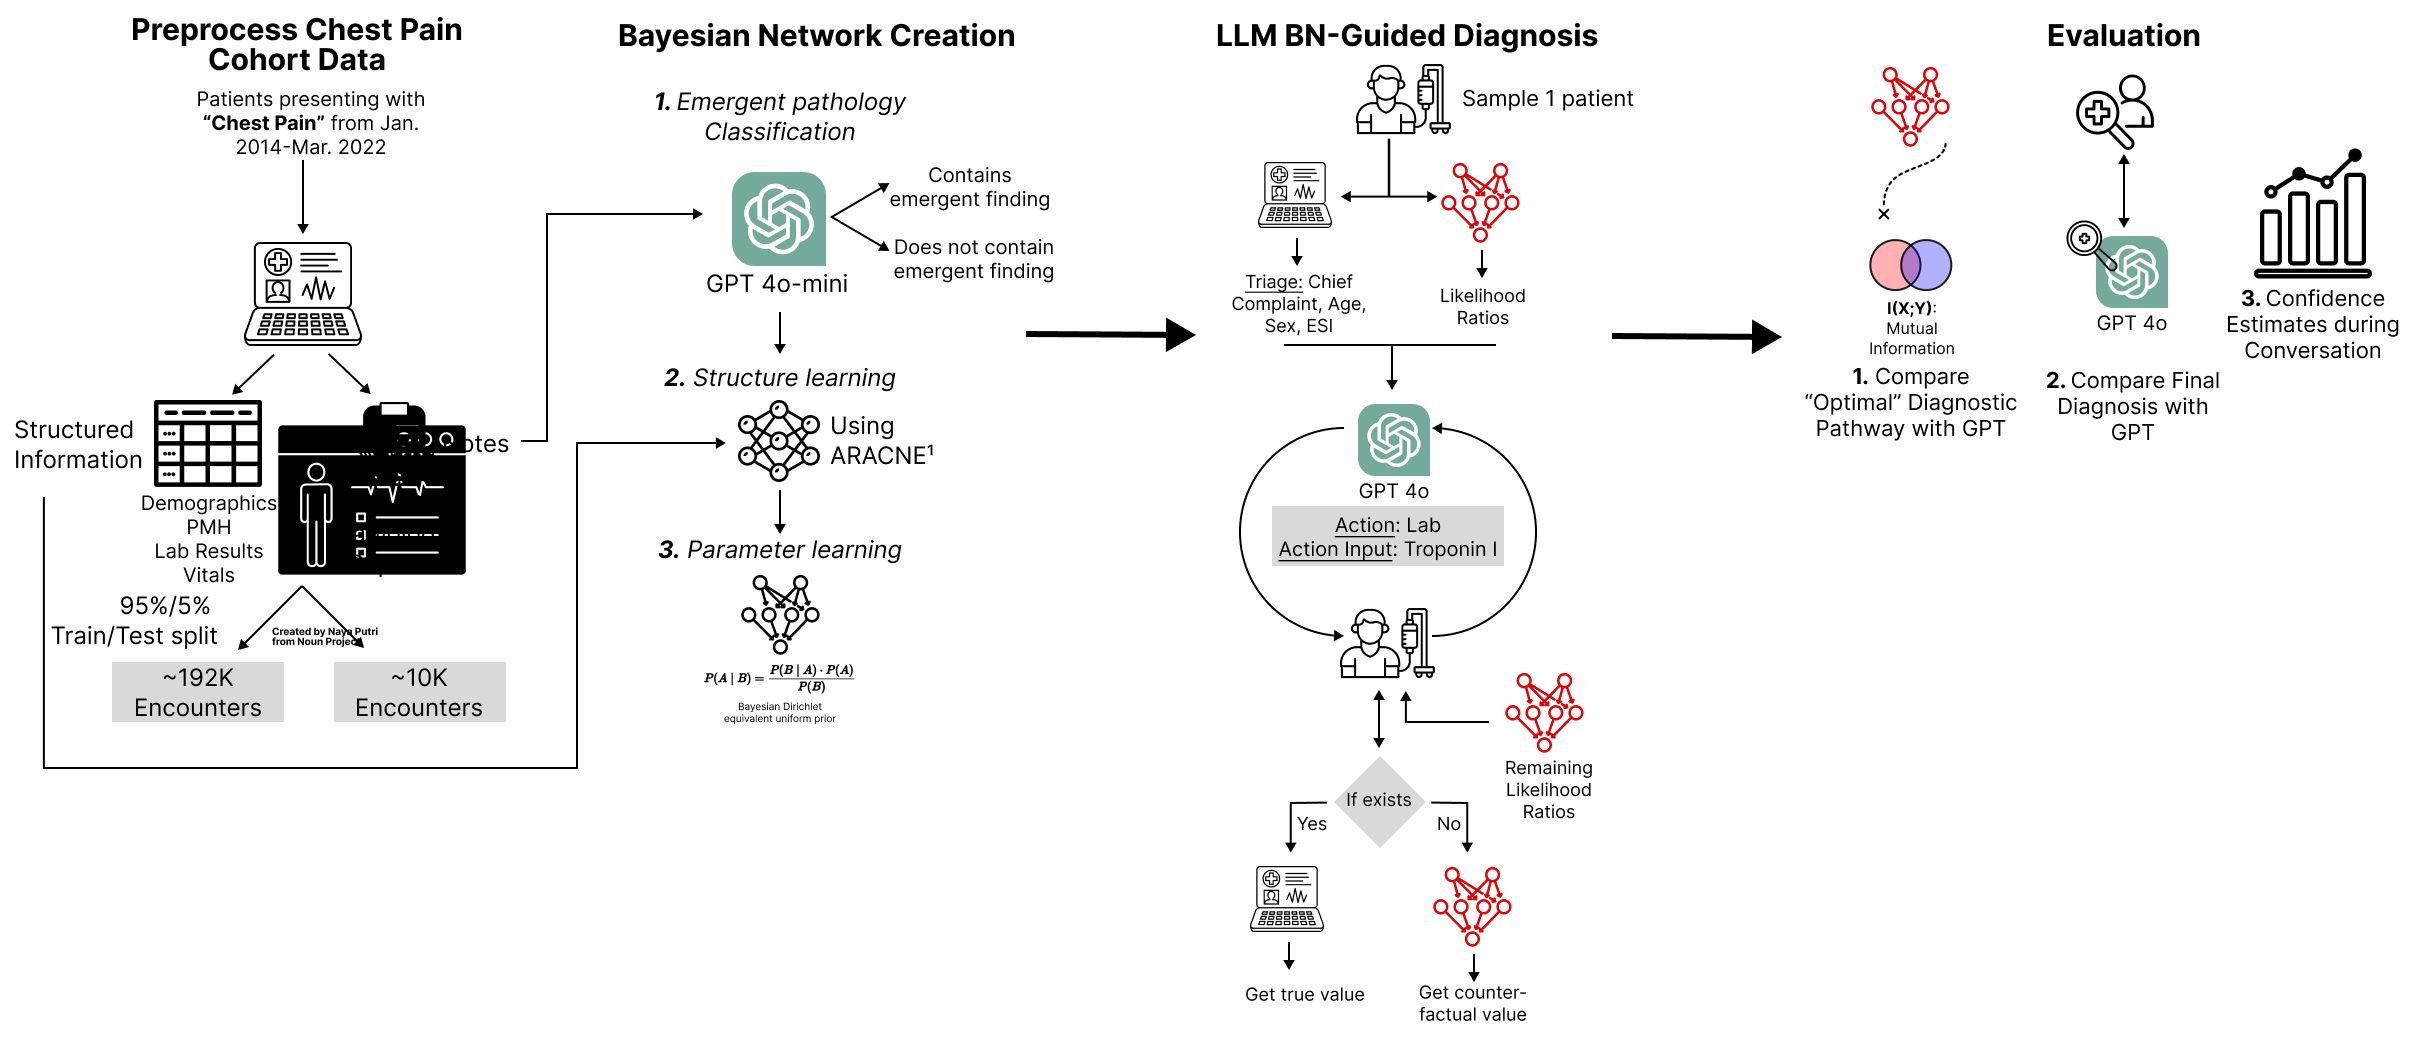
\includegraphics[width=1\textwidth] {figures/aim3/methods_overview.png}
	\caption{Overview of diagnostic conversational evaluation framework, including training of Bayesian Network and comparison to mutual-information optimal diagnostic pathway.} \label{fig:aim3-overview}
\end{figure}

\subsection{Data and Preprocessing}

Our cohort of interest consisted of all encounters for adult patients arriving to the ED at YNHH from January 2014 to April 2022 with a chief complaint of chest pain. We selected 8 emergent/life-threatening diagnoses of interest based on a review of current guidelines and clinical resources (shown in Table 1). All patients were classified as having one of these diagnoses based on the primary diagnosis at disposition, or \emph{Other Diagnosis}. We then preprocessed the available clinical data, including demographics (age, sex, race, smoking status, and Emergency Severity Index [ESI]), past medical history (PMH), laboratory results, vital signs, and imaging findings. All demographic variables, except age, were treated as categorical. ICD-9 codes from the PMH were mapped to the Agency for Healthcare Research and Quality (AHRQ) Clinical Classification Software (CCS) categories \citep{hcup2021ccsr}. The top 15\% most frequent conditions, verified for quality through visual inspection, were selected to capture the most relevant PMH entries. Similarly, only the most frequently recorded laboratory results were included to minimize data quality issues and focus on the most salient data elements. However, unlike demographics and PMH, labs required additional preprocessing. We include lab values that were recorded in $\geq$ 1\% of patients, as well as Troponin values, a significant component of the chest pain diagnostic pathway (e.g. HEART score). All frequent lab types were numeric, so we select the first value recorded during the encounter. For Troponin values, as trends are important in chest pain diagnostic pathways\citep{appleIFCCEducationalMaterials2015}, we identify both the initial Troponin value as well as the change ($\Delta$) between the second and first Troponin values for patients that have multiple values. We also select the first vitals recorded during the encounter, including pulse, SpO2, BP, respiratory rate, temperature, as well as the device used for oxygen therapy, if any. We split our full cohort of patients into a randomized, stratified training (95\%) and test (5\%) set.  Following all preprocessing, our dataset consists of 136 total variables. 

\begin{table}
\centering
\caption{Basic Demographics of Chest Pain Cohort used in GPT 4o Diagnostic Conversations}
\resizebox{0.85\textwidth}{!}{%
\begin{tabular}{llll}
\toprule
 &  & Missing & Overall \\
\midrule
Encounters &  &  & 202632 \\
Patients &  &  & 127338 \\
\cline{1-4}
\multirow[t]{3}{*}{Sex, n (\%)} & Female & 0 & 109148 (53.87) \\
 & Male &  & 93480 (46.13) \\
 & Unknown &  & 4 (0.00) \\
\cline{1-4}
\multirow[t]{7}{*}{Race, n (\%)} & American Indian or Alaska Native & 98 & 788 (0.39) \\
 & Asian &  & 3067 (1.51) \\
 & Black or African American &  & 52596 (25.97) \\
 & Native Hawaiian or Other Pacific Islander &  & 543 (0.27) \\
 & Other &  & 34879 (17.22) \\
 & Unknown &  & 2084 (1.03) \\
 & White or Caucasian &  & 108577 (53.61) \\
\cline{1-4}
\multirow[t]{3}{*}{Ethnicity, n (\%)} & Hispanic or Latino & 0 & 46179 (22.79) \\
 & Non-Hispanic &  & 155216 (76.60) \\
 & Unknown &  & 1237 (0.61) \\
\cline{1-4}
\multirow[t]{5}{*}{Smoking Status, n (\%)} & Former Smoker & 783 & 54667 (27.08) \\
 & Heavy Tobacco Smoker &  & 31379 (15.55) \\
 & Light Tobacco Smoker &  & 8976 (4.45) \\
 & Never Smoker &  & 84601 (41.91) \\
 & Unknown &  & 22226 (11.01) \\
\cline{1-4}
\multirow[t]{2}{*}{CC: Abd. Pain, n (\%)} & 0 & 0 & 190998 (94.26) \\
 & 1 &  & 11634 (5.74) \\
\cline{1-4}
\multirow[t]{2}{*}{CC: Cough, n (\%)} & 0 & 0 & 189469 (93.50) \\
 & 1 &  & 13163 (6.50) \\
\cline{1-4}
\multirow[t]{2}{*}{CC: Dizziness, n (\%)} & 0 & 0 & 192407 (94.95) \\
 & 1 &  & 10225 (5.05) \\
\cline{1-4}
\multirow[t]{2}{*}{CC: Nausea, n (\%)} & 0 & 0 & 191784 (94.65) \\
 & 1 &  & 10848 (5.35) \\
\cline{1-4}
\multirow[t]{2}{*}{CC: Shortness of Breath, n (\%)} & 0 & 0 & 166566 (82.20) \\
 & 1 &  & 36066 (17.80) \\
\cline{1-4}
\multirow[t]{2}{*}{History of Atherosclerosis/Other Heart Dx, n (\%)} & 0.0 & 15808 & 143649 (76.89) \\
 & 1.0 &  & 43175 (23.11) \\
\cline{1-4}
\multirow[t]{2}{*}{History of Diabetes Mellitus, n (\%)} & 0.0 & 15808 & 126048 (67.47) \\
 & 1.0 &  & 60776 (32.53) \\
\cline{1-4}
\multirow[t]{2}{*}{History of HTN, n (\%)} & 0.0 & 15808 & 95307 (51.01) \\
 & 1.0 &  & 91517 (48.99) \\
\cline{1-4}
\multirow[t]{2}{*}{History of Upper Resp. Dx, n (\%)} & 0.0 & 15808 & 141140 (75.55) \\
 & 1.0 &  & 45684 (24.45) \\
\cline{1-4}
\multirow[t]{2}{*}{History of URI, n (\%)} & 0.0 & 15808 & 125730 (67.30) \\
 & 1.0 &  & 61094 (32.70) \\
\cline{1-4}
Creatinine, median [Q1,Q3] &  & 34472 & 0.87 [0.70,1.07] \\
\cline{1-4}
hs Troponin T, median [Q1,Q3] &  & 198659 & 8.00 [6.00,16.00] \\
\cline{1-4}
Troponin I, median [Q1,Q3] &  & 153290 & 0.01 [0.01,0.02] \\
\cline{1-4}
Troponin T, median [Q1,Q3] &  & 174492 & 0.01 [0.01,0.01] \\
\cline{1-4}
\multirow[t]{4}{*}{ECG, n (\%)} & Emergent Pathology & 0 & 216 (0.11) \\
 & No Emergent Pathology &  & 3747 (1.85) \\
 & No Test Ordered &  & 6311 (3.11) \\
 & Ordered Test &  & 192358 (94.93) \\
\cline{1-4}
\multirow[t]{4}{*}{CT Abdomen, n (\%)} & Emergent Pathology & 0 & 368 (0.18) \\
 & No Emergent Pathology &  & 889 (0.44) \\
 & No Test Ordered &  & 196069 (96.76) \\
 & Ordered Test &  & 5306 (2.62) \\
\cline{1-4}
\multirow[t]{4}{*}{CT Chest, n (\%)} & Emergent Pathology & 0 & 125 (0.06) \\
 & No Emergent Pathology &  & 122 (0.06) \\
 & No Test Ordered &  & 201168 (99.28) \\
 & Ordered Test &  & 1217 (0.60) \\
\cline{1-4}
\multirow[t]{4}{*}{XR Chest, n (\%)} & Emergent Pathology & 0 & 3098 (1.53) \\
 & No Emergent Pathology &  & 50283 (24.81) \\
 & No Test Ordered &  & 37063 (18.29) \\
 & Ordered Test &  & 112188 (55.37) \\
\cline{1-4}
\multirow[t]{4}{*}{Echo, n (\%)} & Emergent Pathology & 0 & 147 (0.07) \\
 & No Emergent Pathology &  & 512 (0.25) \\
 & No Test Ordered &  & 171592 (84.68) \\
 & Ordered Test &  & 30381 (14.99) \\
\cline{1-4}
\multirow[t]{8}{*}{Primary Diagnosis, n (\%)} & Acute Coronary Syndrome & 0 & 2099 (1.04) \\
 & Aortic Dissection &  & 133 (0.07) \\
 & Esophageal Rupture &  & 13 (0.01) \\
 & Other Diagnosis &  & 198286 (97.86) \\
 & Pericarditis &  & 192 (0.09) \\
 & Pneumonia &  & 529 (0.26) \\
 & Pneumothorax &  & 260 (0.13) \\
 & Pulmonary Embolism &  & 1120 (0.55) \\
\cline{1-4}
\bottomrule
\end{tabular}

\label{tab:aim3-table1}
}
\end{table}

\subsection{Emergent Pathology Classification of Imaging Consults}

Since Bayesian networks (BNs) require categorical input data, free-text information, such as imaging consult reports, was processed and classified into discrete categorical variables. Given the large number of potential outcomes associated with various diagnostic tests relative to the size of our cohort, we simplified the categorization of imaging consult reports to just indicate the presence of any emergent finding. This approach allowed us to focus on clinically significant outcomes while reducing the dimensionality of the data. To do so, we first extracted all available radiology reports associated with our cohort. Due to computational constraints, the number of imaging consult notes extracted was limited (66,205 notes, 14.74\% of total consults). However, for cases where the radiology report was not available, the LLM was still provided with the information that a consult was ordered. All available radiology reports were de-identified using a custom pipeline for YNHH notes. Following de-identification, imaging order types were categorized based on modality and their relevance to chest pain-related diagnoses, grouping them into categories such as "CT\_Chest" (directly related to chest pain) and "CT\_Other" (e.g. abdominal CT). We identified a total of 7 imaging categories, described in Appendix \ref{tab:aim3-data-
columns}.

In order to classify radiology consults as containing an emergent finding, a black-box LLM, GPT 4o-mini, was queried. Our initial testing showed that while GPT 4o-mini performed marginally worse in classification, the cost of classifying all documents was significantly lower. Following classification by the LLM, each imaging modality had four possible outcomes for a patient: \emph{no test ordered}, \emph{test ordered, unknown result}, \emph{test ordered, no emergent finding}, \emph{test ordered, emergent finding}. We report the performance of GPT 4o-mini on a small evaluation set in the Appendix (Figure~\ref{fig:aim3-imaging-path-confmat}). 

\subsection{Derivation of the Bayesian Network}

All preprocessed clinical history in our training set was used to train a Bayesian network. Prior to training, to generate categorical variables, continuous data was binned into 5 equal interval width bins. Upon initial testing, it was identified that Troponin values, and in particular Troponin $\Delta$ ranges were too large to be clinically meaningful. Therefore, instead of equal width bins, reference ranges were identified and used for these values instead \cite{americanboardofinternalmedicineLaboratoryreferenceranges2024, diercksDiagnosticAccuracyPointofcare2012, pirruccelloHSTroponinInterpretation, storrowAbsoluteRelativeChanges2015, vallabhajosyulaRoleAdmissionTroponinT2017}. 

The Bayesian network structure was trained using the ARACNE algorithm \citep{margolinARACNEAlgorithmReconstruction2006}, a constraint-based approach. This method was chosen because most score-based algorithms require complete datasets without missing values. By contrast, the constraint-based approach allows us to capture the clinical significance of missing data, such as the absence of an ordered test reflecting a deliberate clinical judgment. The ARACNE algorithm first estimates pairwise mutual information (MI) between all variables. Then, it sets a threshold based on the p-value of a null hypothesis of independence to determine the initial set of edges to exist in the network. To address the potential for highly correlated variables mediated by a third concept, which can result in false positives (e.g. dizziness/vomiting → nausea/vomiting vs. dizziness/vomiting $\rightarrow$ headache/migraines $\rightarrow$ nausea/vomiting), the second step of the algorithm employs the Data Processing Inequality (DPI) to eliminate spurious direct connections. This algorithm provided an undirected graph with likely relationships between variables of interest. We then set the directionality using the topological ordering provided by the \emph{dot} algorithm, assuming reciprocal directed edges between all nodes. To validate the structure of the Bayesian network, we sampled random walks covering 50\% of the network nodes. Two ED physicians manually reviewed the relationships within these chains and the proportion of valid connections was recorded. Once the network structure was validated, the conditional probabilities between connected nodes were trained using the maximum likelihood estimator (MLE). We also present the classification performance of the trained BN on the 7 emergent findings of interest. 

\subsection{LLM Diagnostic Conversations}

As shown in Figure \ref{fig:aim3-overview}, after training the Bayesian network (BN), the LLM is tasked with conducting diagnostic conversations with chest pain patients. We select a convenience sample of 500 patients, given multiple evaluation conditions and cost constraints. During these interactions, the LLM is provided with requested information if it is available. For cases where the requested information is unavailable, the BN is utilized to infer the most likely outcome for the specific patient profile. The encounter with the LLM began with a brief introduction to the patient including information conventionally recorded at triage (i.e. chief complaint, age, sex, and ESI level). We opted to limit the initial information provided to ensure that the LLM was not biased in its information seeking. Following this initial presentation, the LLM was provided with a list of available information to choose from. Following \citet{hagerEvaluationMitigationLimitations2024}, we design a prompt that requires the LLM to request both the information type (e.g. \emph{"lab value"}) and the specific piece of information (e.g. \emph{"1st Troponin I"}), shown in Figure \ref{fig:aim3-prompt}. If a structured element is requested, we record whether the request was valid and if so, provide the LLM with the structured information, including units (e.g. \emph{"0.4 ng/mL"}). For a free text request, in the event that the consult was ordered and we are missing the radiology note, we encourage the LLM to consider the reasoning associated with the original physician's decision to request the consult by responding \emph{"ED physician determined the test was indicated and the test was ordered; unknown result."}. If the note exists within the dataset, it is provided instead. All orders that do not exist in our dataset are assumed to have not been ordered to simplify decision making. At any point, the LLM can decide that it has gathered enough information and select a diagnosis from the list of 7 life-threatening conditions, or "Other Diagnosis" assuming none of the diagnoses of interest. The maximum number of conversational turns was set to 39, reflecting the average number of informational elements requested by physicians during the original clinical encounters. If the LLM reaches 39 requests, it is forced to assign a diagnosis.

In addition to the structured evaluation, where the LLM selects from a predefined set of diagnoses, we also investigated the effects of disease prevalence and prompt context on diagnostic performance. To achieve this, we designed two additional prompting strategies. Initial testing revealed that the LLM assigned diagnoses of interest far more frequently than expected based on their actual prevalence. Recognizing that these life-threatening conditions are rare, we incorporated prevalence information into the prompts to recalibrate the LLM, guiding it to better align its diagnostic predictions with realistic probabilities. Additionally, we designed a neutral prompt that avoided biasing the LLM toward any specific set of diagnoses. For this final prompt, each condition was manually classified into one of the eight diagnoses of interest to enable consistent, direct comparisons across evaluation methods. % Finally, to enhance the probabilistic reasoning available to the LLM, we queried the Bayesian network (BN) for likelihood ratios (LRs) of all diagnostic tests based on the patient's current clinical data. The LRs were defined as: "the probability of a person who has the disease testing positive divided by the probability of a person who does not have the disease testing positive" (Equation \ref{eq:aim3-LR}). The top five LRs were provided to the LLM, enabling it to integrate its clinical reasoning with probabilistic insights from the BN when determining which piece of information to request next.

We assessed the relative performance of all three prompting strategies using confusion matrices and compared the LLM's diagnostic accuracy to the original primary diagnosis. Additionally, we derived an "optimal" diagnostic pathway using mutual information (MI) principles from the BN. At each diagnostic step, we identified the information element with the highest average MI across all potential diagnoses, establishing a decision-analytic benchmark. The sequence of information requests made by the LLM was then compared to this "optimal" approach using rank-biased overlap (RBO), a common metric used in recommendation systems such as search engines that emphasizes earlier elements more than latter ones\citep{webberSimilarityMeasureIndefinite2010}. We chose this metric as selecting the first few diagnostic tests correctly is more important as the diagnostic decision space is broad and uncertainty is high. Clinically, further tests are largely used for confirmation and therefore are less significant. Furthermore, we analyzed the total number of information elements requested by the LLM in comparison to those requested by the original physician. Finally, we evaluated the internal model of uncertainty in the LLM as a function of the diagnostic narrowing task. At each conversation turn, we prompt the LLM to provide both its requested next action, as well as the likelihood of each of the diagnoses of interest (in the constrained prompting strategy). We present the distribution of maximum confidences for any one of the diagnoses across the test cohort of 500 patients at each conversation turn. % Finally, we evaluated the relative diagnostic costs associated with the full set of information requests for both the LLM and the physician to determine which approach incurred higher per-patient costs.

We first present results of the Bayesian network training process, followed by performance comparing the various prompting strategies compared to the diagnosis of the physician from the original encounter, as well as compared to the MI-biased optimal sequence of diagnostic tests. Finally, we present the confidence distributions at each step in the conversation.  

\section{Results}
We first present the performance of the trained Bayesian Network on classification as validation of the conditional probability tables (CPDs) (Figure~\ref{fig:aim3-bn-confmats}). In general, the likelihood of even the most frequent emergent pathology (ACS) is very low, 1.0\%. The Bayesian network has a significant number of false positives in the 3 most frequent conditions (ACS, PE, and Pneumonia), leading to poor F1-scores (range: $[0.018-130]$). However, recall was the highest of all diagnoses for ACS (0.714). The weighted macro-averaged F1-score across all conditions is 0.046. Recall, a more critical metric for identifying relevant diagnostic tests for life-threatening "can't-miss" conditions, achieves a higher performance of 0.475. 

\begin{figure}[H]
	\centering
	\includegraphics[width=0.85\textwidth] {figures/aim3/bn_confmats.png}
	\caption{Confusion matrices of trained Bayesian network compared to primary diagnosis from original encounter on test set.} \label{fig:aim3-bn-confmats}
\end{figure}


We next compare the performance of the three prompting strategies on the oversampled evaluation set of 500 patients: including a finite set of diagnoses, including the low prevalence of emergent findings, and finally with no restrictions on diagnoses of interest. We represent the results as differences between the confusion matrices. As shown in Figure~\ref{fig:aim3-diff-confmat}, the impact of including the low prevalence of life-threatening conditions reduces the number of false positives of ACS ($\Delta=-11\%$) and increases the true positive identification of "Other Diagnoses" ($\Delta=+21\%$). However, it also increases the number of false positive "Other Diagnosis" predictions across all categories. These trends are amplified when no restrictions are placed on diagnoses of interest, as the increase in correct diagnoses of "Other Diagnosis" is larger ($\Delta=+28\%$), while the false positives of conditions like ACS and PE have also increased ($+16\%$ and $+8.2\%$, respectively).

\begin{figure}[H]
	\centering
	\includegraphics[width=\textwidth] {figures/aim3/diff_confmat_GPT.png}
	\caption{Comparison of confusion matrices illustrating the diagnostic accuracy differences between GPT-4 and the physician from the original encounter across three prompting strategies. The original approach, where the LLM was constrained to select from a predefined set of diagnoses, is compared to two alternative strategies: incorporating prevalence data (left) and providing no information about specific diagnoses of interest (right).} \label{fig:aim3-diff-confmat}
\end{figure}

We further compare the performance against the mutual-information-based optimal performance using the RBO. We represent the overlap on a scale of $0-1$ to demonstrate the relatively low overlap between GPT and the physician from the original encounter. The diagnosis with the highest overlap was pneumonia (0.097) and the lowest was pericarditis (0.060), with no significant differences in the amount of overlap between the diagnoses of interest. 

\begin{figure}[H]
	\centering
	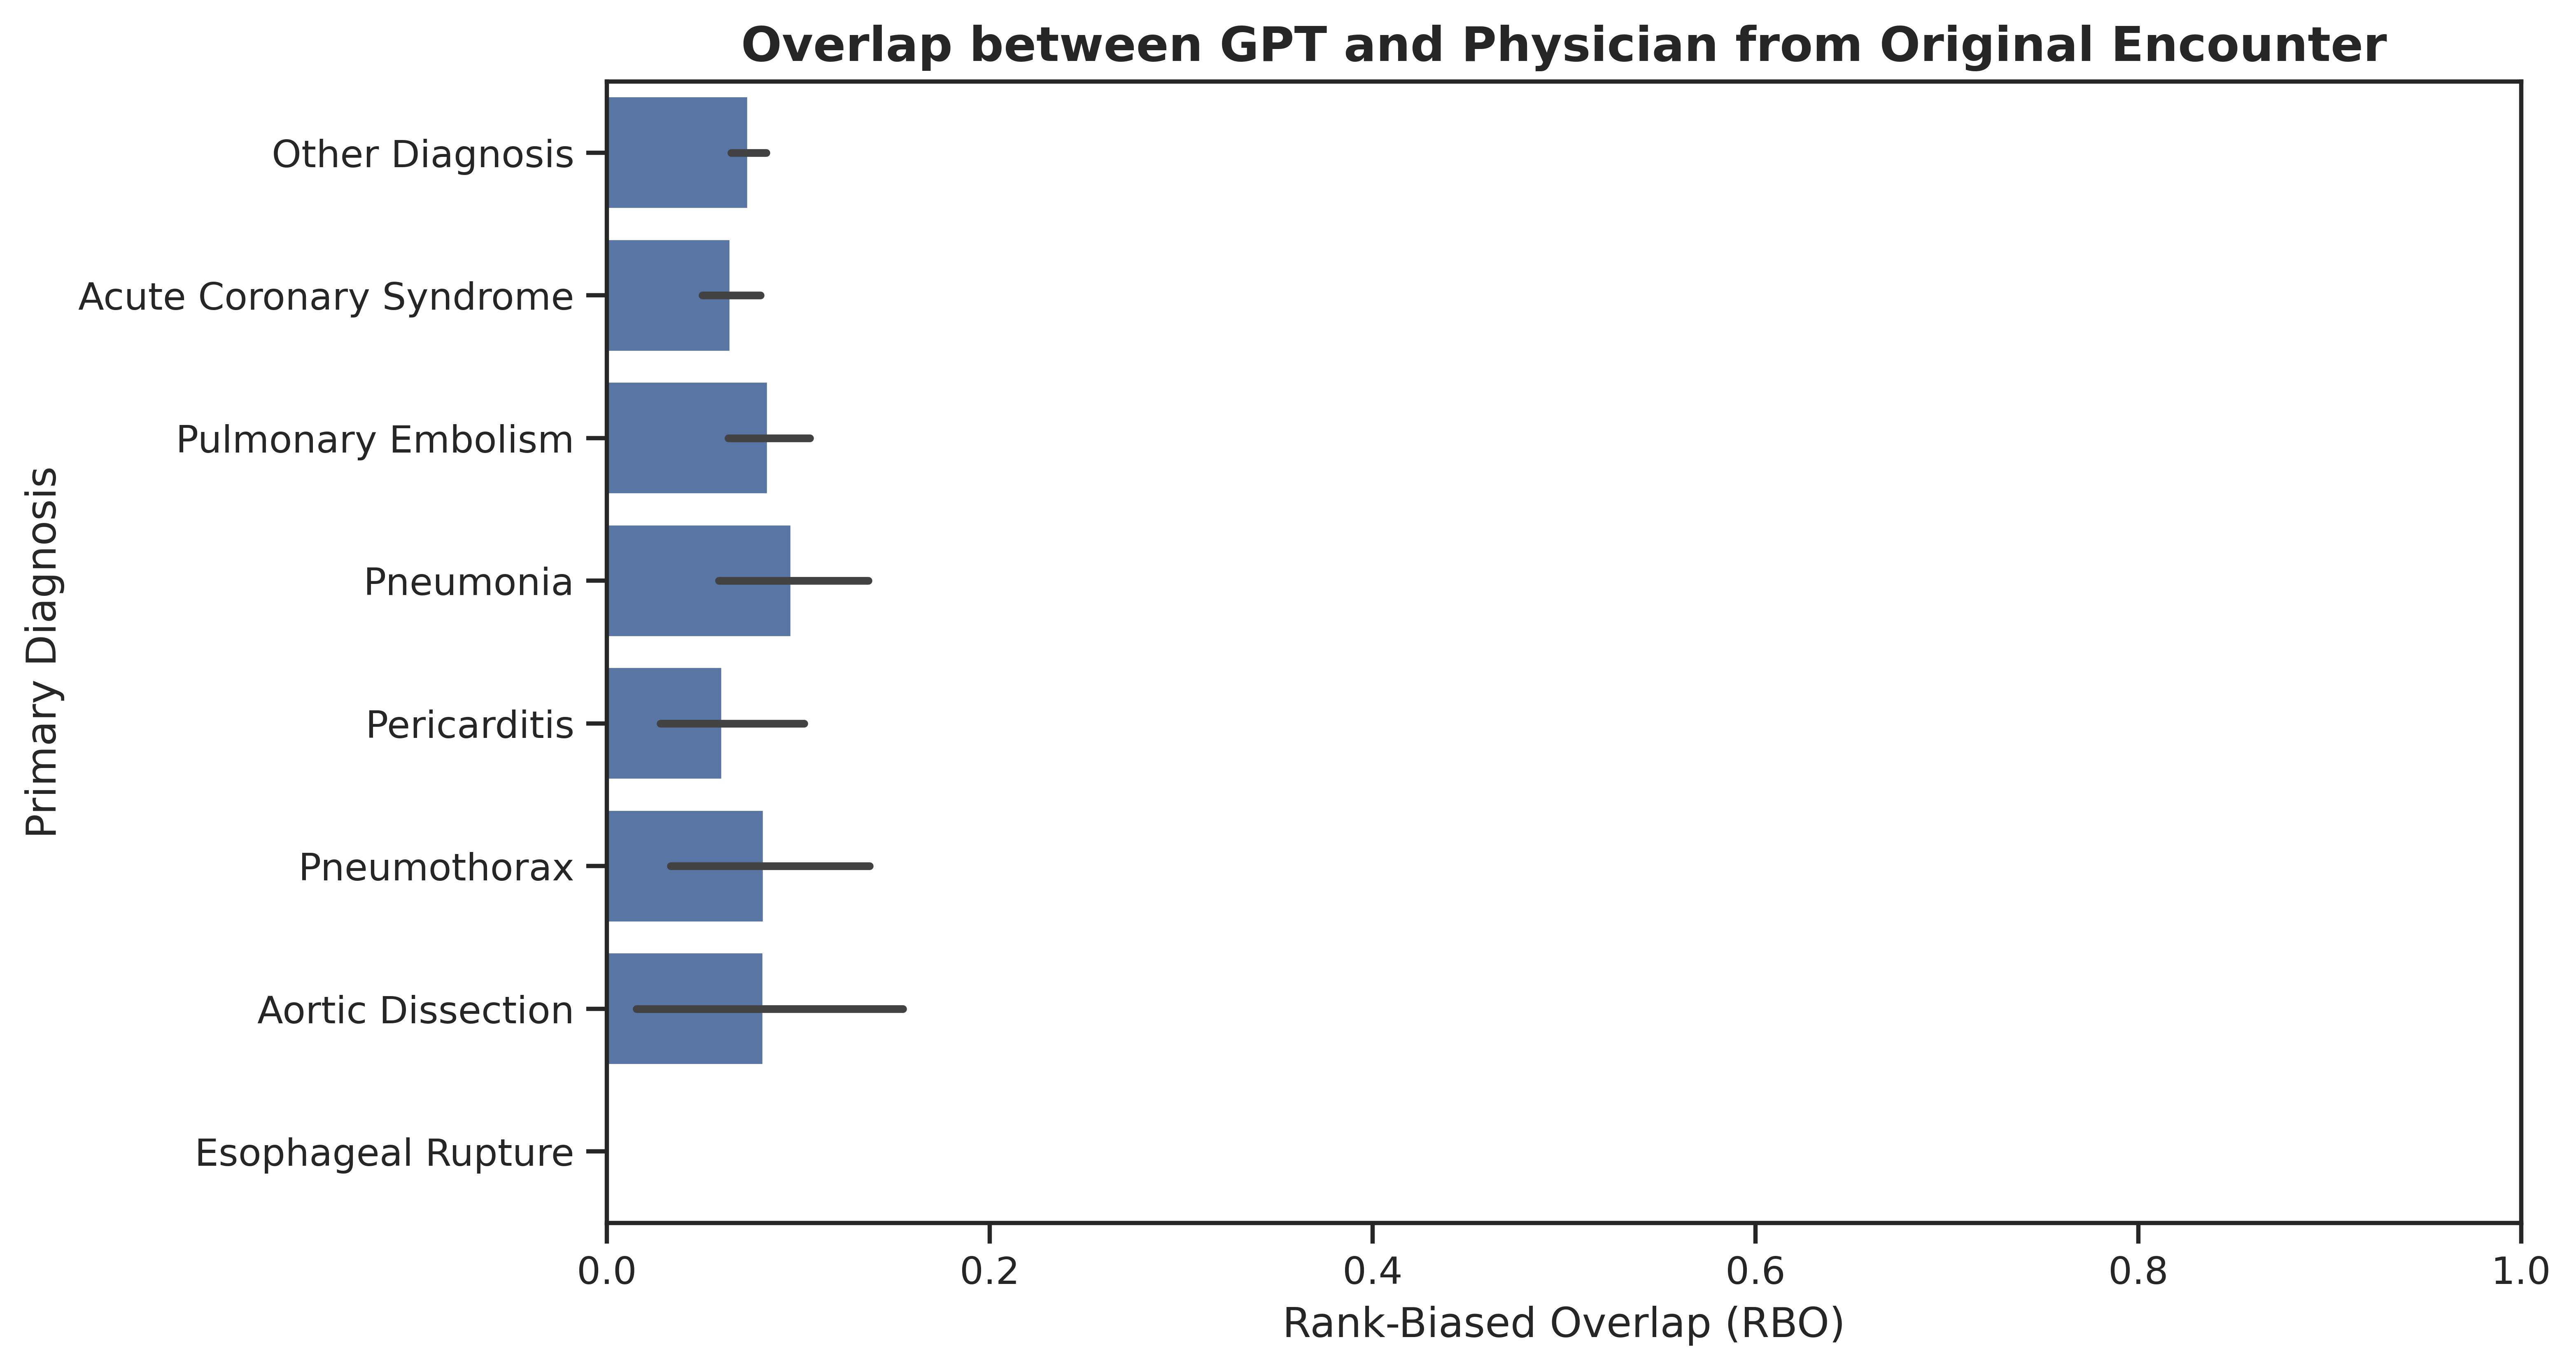
\includegraphics[width=\textwidth] {figures/aim3/optimal_overlap.png}
	\caption{The rank-biased overlap (RBO) between the physician from the primary encounter and GPT. Given the small fraction of tests requested of those available, we use the extension of RBO in which the degree of agreement seen up to depth $k$ is continued indefinitely to measure the full potential overlap if more diagnostic tests were requested.} \label{fig:aim3-optimal-overlap}
\end{figure}

We compare not only the diagnostic performance of the LLM to that of the physician from the original encounter, but also the number of data elements requested by both (Figure~\ref{fig:aim3-data-types}). We see that when compared to the three prompting strategies, physicians request the most amount of information by a significant margin in both vitals and lab values. However, the LLM requests more imaging information by a significant margin. There are only minor differences between the three prompting strategies, although in most cases, when GPT is provided the diagnoses of interest, it requests less information of all types except imaging. 

\begin{figure}
    \centering
	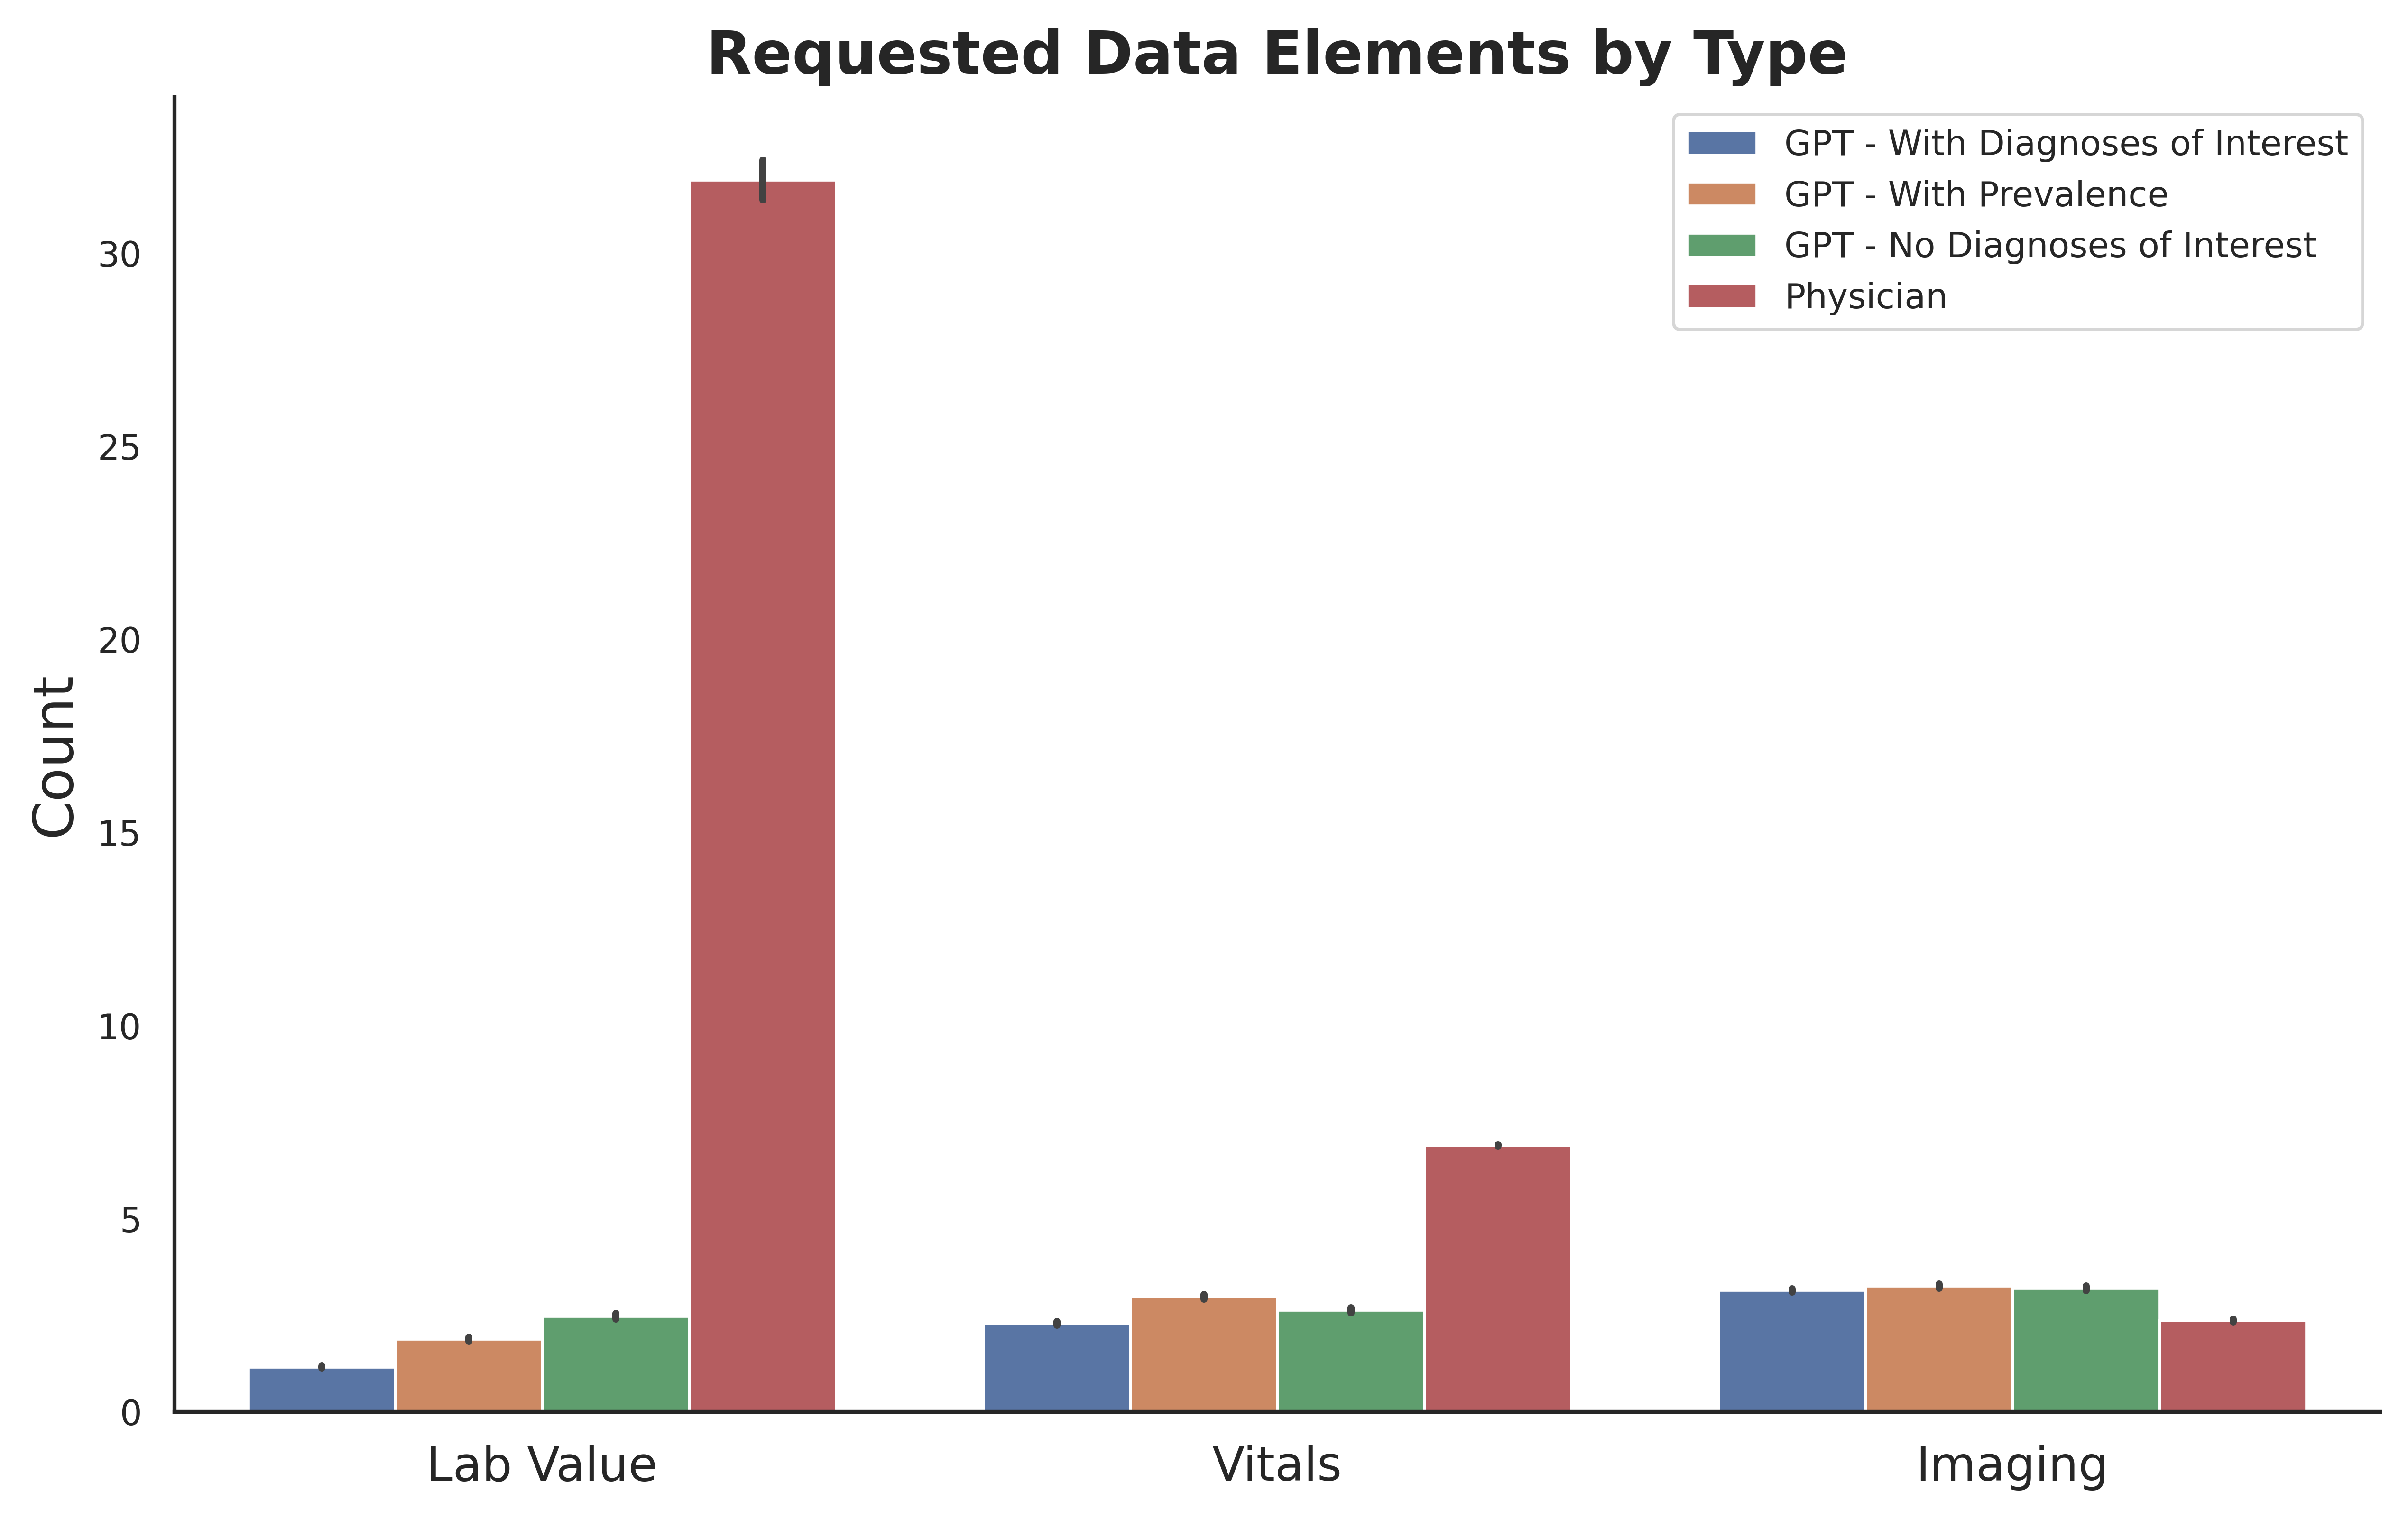
\includegraphics[width=0.6\textwidth] {figures/aim3/requested_data_by_type.png}
	\caption{Comparison of number of data elements requested by LLM and physician from original encounter by data type.} \label{fig:aim3-data-types}
\end{figure}    

Finally, we aim to evaluate whether LLMs effectively emulate the diagnostic narrowing process observed in physicians, refining a diagnosis with increasing specificity. We present a ridgeline plot of the distribution of maximum confidence for any diagnosis of interest at each step in the conversation. We notice that across the 40 diagnosis steps, in general, the average max confidence increases until step 12 and then remains approximately static until decreasing from steps 24-32, before rising again until the end of the conversation (Figure~\ref{fig:aim3-confidence-steps}). The distributions towards the end of the conversation also have a higher variance compared to those earlier on in the conversation. 

\begin{figure}[H]
    \centering
	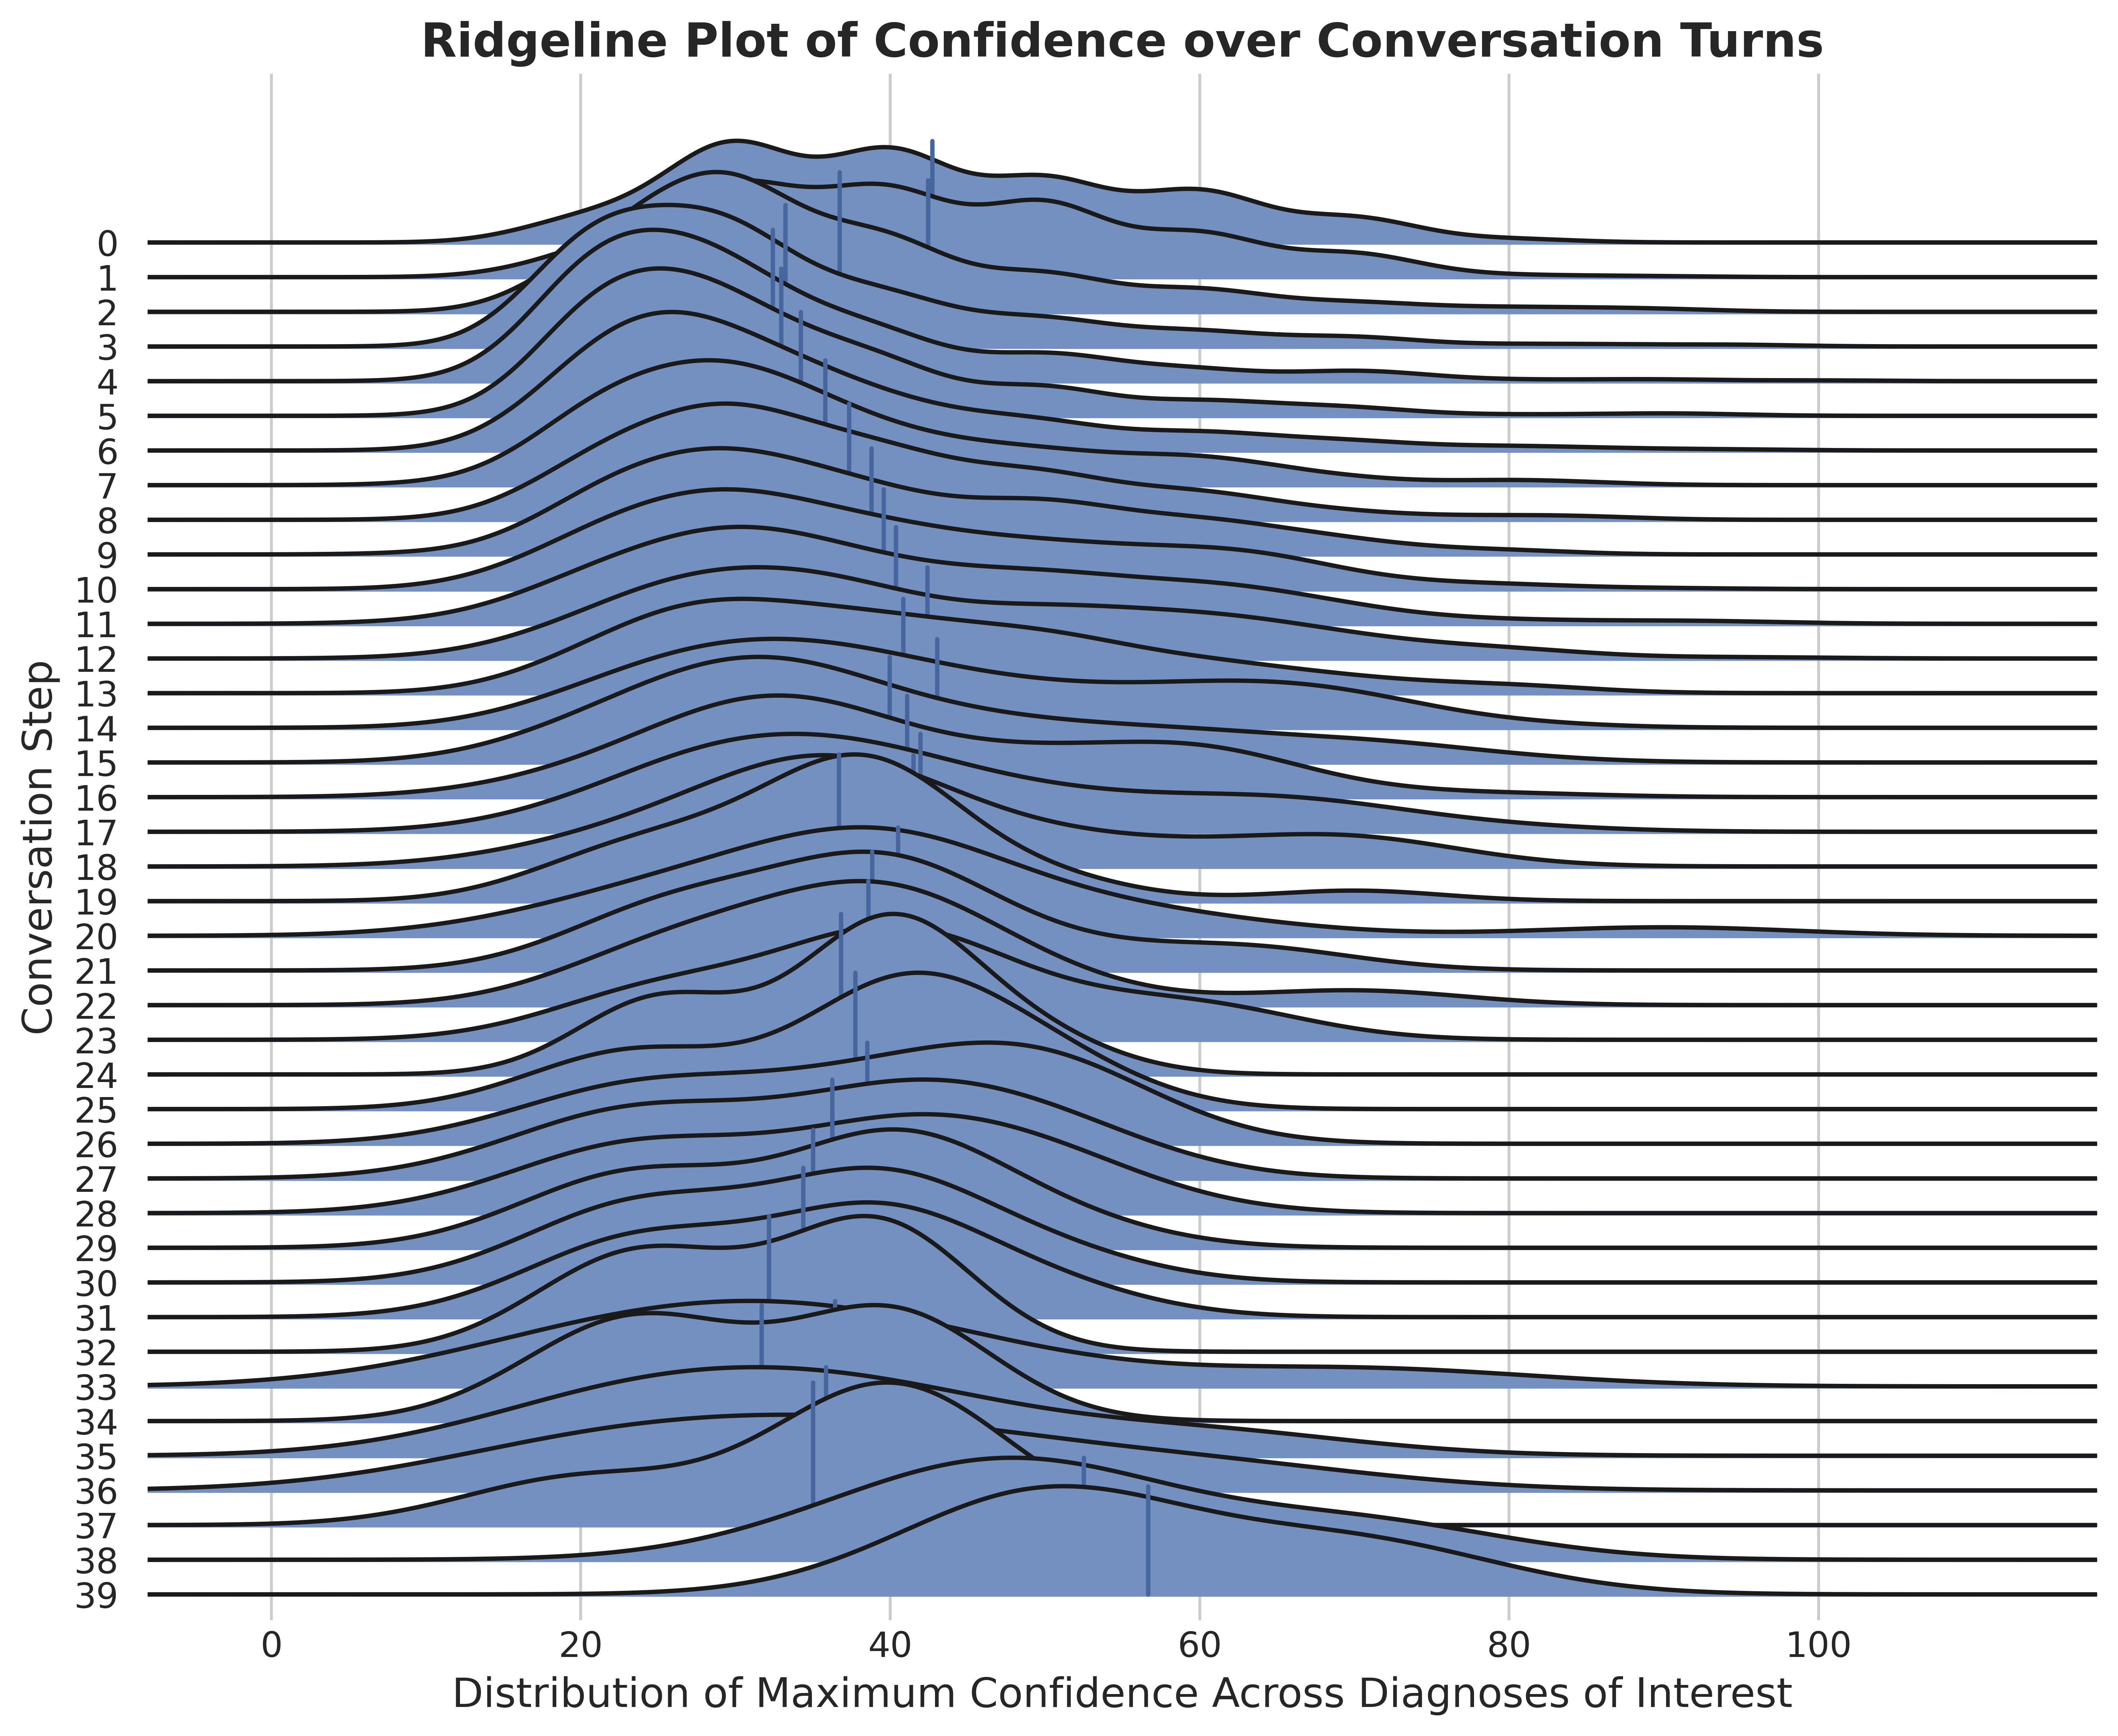
\includegraphics[width=\textwidth] {figures/aim3/confidence_over_steps.png}
	\caption{A ridgeline plot describing the distribution of max confidence values over all diagnoses of interest on the evaluation cohort.} \label{fig:aim3-confidence-steps}
\end{figure}    

\section{Discussion}
In this work, we evaluate a state-of-the-art LLM (GPT-4o) in conducting diagnostic conversations with chest pain patients arriving in the emergency department (ED), backed by a Bayesian network trained on a cohort of YNHH patients. The Bayesian network was used to both introduce missing information into the LLM input, as well as to evaluate against as a mutual-information-based optimal diagnostic pathway. We conduct conversations using three prompting strategies with various amounts of probabilistic information. As a baseline, we prompt the LLM to select between 7 different emergent pathologies, or "Other Diagnosis" if none of the relevant diagnoses apply. However, on initial testing, we found that the LLM overestimates the likelihood of diseases of interest, despite their low real-world prevalences. To assess the impact of the LLM's role on diagnostic performance, we evaluate two more prompting strategies: incorporating prevalence data and eliminating restrictions on the range of final diagnoses the LLM can select. For the latter, we manually align the generated diagnoses with our predefined set of eight target diagnoses. Finally, we compare all prompting strategies to the primary diagnosis from the physician from the original encounter as well as the MI-based "optimal" pathway. Lastly, we compare the amount of information requested by the LLM and the physician, as well as the changing confidence distributions at various steps of the conversation. 

In general, we find that the LLM overestimates the likelihood of low-prevalence conditions when guided or influenced towards specific diagnoses of interest. This is somewhat ameliorated by the inclusion of prevalence data in the system role and prompt. False positives of diagnoses of interest are further reduced when no restrictions are placed on the diagnoses of interest the LLM can select. However, this setting led to an increase of false positive classifications of "Other Diagnosis" suggesting that excessive freedom causes the LLM to misinterpret clinical features, leading to a lack of focus in identifying diagnostically meaningful patterns aligned with a clinical objective. This conclusion is further supported by the unclear and nonspecific free-text diagnoses assigned by the LLM (e.g. \emph{Anemia contributing to hypoxemia and elevated troponin due to systemic effects} or \emph{Chest pain related to anxiety disorder}). 

When comparing the LLM to the MI-based "optimal" approach, there was very low overlap between the LLM's selected set of diagnostic tests and that of the Bayesian network. In a qualitative evaluation, we noticed that some form of Troponin testing was requested by the LLM early in the diagnostic conversation ($\leq4$ steps), whereas in some cases, the "optimal" approach suggests that the Troponin test should come later (between 8-10 conversation steps). Similarly, one of the first few requests was for imaging, as compared to the optimal pathway when imaging appeared later. Assuming the optimal diagnostic pathway is similar to the one that the physician from the original encounter chose, this latter conclusion is supported by our investigation into the number of data elements requested by type in which GPT requested significantly more imaging than the physician. However, the physician requested significantly more of both other types of information, lab values and vitals. One potential reason for this is that in the ED, both labs and vitals can be gathered in aggregate (e.g. a CBC/lipid panels and continuous vital signs monitors). As a result, these data elements are considered separate by the LLM, but not by the physician, artificially increasing the number of requests by the physician. 

Finally, we prompt the LLM to provide a likelihood for all diagnoses of interest at each step in its diagnostic conversation. Rather than visualize the distribution of likelihoods for all diagnoses, we instead simply select the highest likelihood under the assumption that there must be a higher proportion of likelihoods at later stages in the diagnostic conversation. While we see this to some degree, there appears to be some variation as conversations progress. More significantly, even at the end of the conversation, the LLM has relatively low confidence ($avg@step\ 40 = 58\%$). We conclude that while there is a slight trend towards increasing confidence in a final diagnosis as conversation continues, the LLM's clinical uncertainty is poorly calibrated and does not align with its diagnostic narrowing process. 

This study does have several limitations. The most significant of which is the poor classification performance achieved by the trained Bayesian network. Due to the very low prevalence (at most 1\%) of all the emergent pathologies of interest, prediction was difficult. Moreover, the model was originally trained to emphasize a clinically meaningful structure, rather than predictive performance because a BN more representative of clinical  pathways is more likely to provide a meaningful order of optimal diagnostic tests in evaluation. However, this focus on a BN structure that modeled clinical practice may not have been the optimal one for diagnosis prediction, lowering performance. Despite the overall poor performance of the BN, we prioritized increasing recall over precision, as the optimal diagnostic path should focus on ruling out life-threatening conditions, even if it results in additional testing. However, this emphasis by the BN conflicted with the LLM's goal of minimizing additional information requests prior to diagnosis, potentially contributing to the low overlap in the elements of information requested by the two systems. The BN may have also suffered in performance due to the lack of important information conventionally available to the physician and necessary in chest pain evaluations: the results of the initial presentation. Including these results may improve both the performance of the BN and the LLM. However, despite these limitations, we revealed significant deviations by the LLM in its diagnostic decision making process from physicians in the evaluation of chest pain. 

Overall, our findings indicate that LLMs tend to overemphasize prompt context, exhibit a limited understanding of real-world clinical probabilities, and demonstrate poorly calibrated confidence. These limitations underscore the need for significant caution when considering the implementation of LLMs as diagnostic chatbots, particularly in patient-facing clinical decision support tools. LLMs currently lack the ability to replicate physician-level or optimal decision-making processes, necessitating substantial oversight in their deployment as diagnostic aids. We hope this study inspires future efforts to advance the development of LLMs that are better aligned with the decision-making frameworks used in clinical practice.

\section{Impact on Theory of Clinical Uncertainty}

This work represents the final step in our development of a theory of clinical uncertainty in large language models (LLMs). In previous chapters, we demonstrated that an LLM's internal representation of uncertainty is highly influenced by both the specific disease context and the assigned role of the LLM. We observed that, when given a task such as deprescribing, the LLM significantly overestimated the likelihood of deprescribing a medication compared to real-world clinical probabilities. Moreover, the model exhibited logical inconsistencies, making recommendations without sufficient supporting evidence, in an effort to fulfill the task. Similarly, in the context of Bayesian diagnostic reasoning, the model showed a limited understanding of real-world clinical probabilities, such as the predictive performance of diagnostic tests. 

In this chapter, similar to our findings from Chapter~\ref{chapter:deprescribing} with deprescribing, the LLM tended to overestimate the likelihood of rare, life-threatening conditions simply because they were emphasized as diagnoses of interest in the prompt. These findings support our hypothesis that LLMs tend to overemphasize the likelihood of events based on contextual cues while failing to appropriately account for real-world probabilities. Providing prevalence data or removing prompt-based contextual biases significantly reduced this overemphasis, highlighting the importance of the context the LLM is placed in. This theory and its conclusions motivate the need for integration of real-world probabilistic knowledge into LLMs, as well as subsequent alignment of the internal model of clinical uncertainty to that of physicians.

